\chapter{Affine Transformations of the Independent Variable (Oppenheim 1.2-1.3)}

\begin{definition}
    [Affine Transformation]
    An \textbf{affine transformation} of the independent variable is a transformation of the form
    \[
        y(t) = x(at + b)
    \]
    where $a$ and $b$ are constants.
\end{definition}

\begin{definition}
    [Time Reversal]
    The \textbf{time reversal} of a signal $x(t)$ is defined as
    \[
        x(t) \to x(-t) = \tilde{x}(t)
    \]
\end{definition}
\begin{figure}[h]
    \centering
    \begin{minipage}{0.45\textwidth}
        \centering
        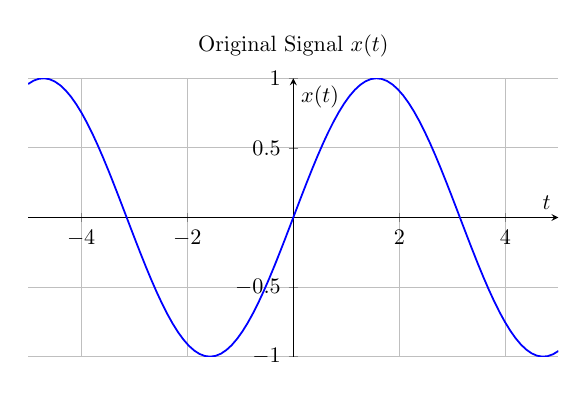
\begin{tikzpicture}[scale=0.8]
            % Original signal x(t)
            \begin{axis}[
                    title={Original Signal $x(t)$},
                    xlabel={$t$},
                    ylabel={$x(t)$},
                    axis lines=middle,
                    grid=both,
                    width=10cm,
                    height=6cm,
                    domain=-5:5,
                    samples=100
                ]
                \addplot[blue, thick] {sin(deg(x))};
            \end{axis}
        \end{tikzpicture}
    \end{minipage}
    \hfill
    \begin{minipage}{0.45\textwidth}
        \centering
        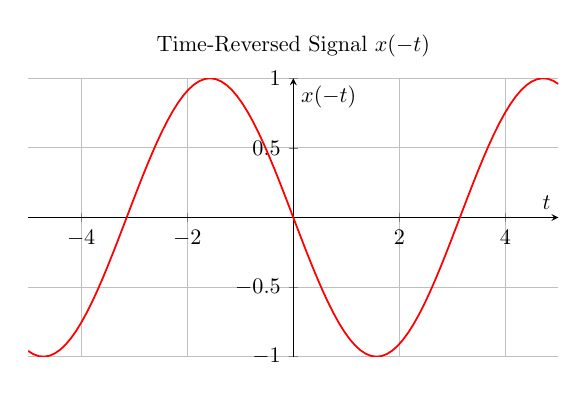
\begin{tikzpicture}[scale=0.8]
            % Time-reversed signal x(-t)
            \begin{axis}[
                    title={Time-Reversed Signal $x(-t)$},
                    xlabel={$t$},
                    ylabel={$x(-t)$},
                    axis lines=middle,
                    grid=both,
                    width=10cm,
                    height=6cm,
                    domain=-5:5,
                    samples=100
                ]
                \addplot[red, thick] {sin(deg(-x))};
            \end{axis}
        \end{tikzpicture}
    \end{minipage}
    \caption{Time Reversal of a Signal}
    \label{fig:time-reversal}
\end{figure}

\begin{definition}
    [Time Dilations]
    The \textbf{time dilation} of a signal $x(t)$ is defined as
    \[
        x(t) \to x(at)
    \]
\end{definition}

\begin{definition}
    [Time Advancement]
    The \textbf{time advancement} of a signal $x(t)$ is defined as
    \[
        x(t) \to x(t - b)
    \]
\end{definition}

\begin{definition}
    [Time Delay]
    The \textbf{time delay} of a signal $x(t)$ is defined as
    \[
        x(t) \to x(t + b)
    \]
\end{definition}

\begin{corollary}
    [Time Dilation in Discrete-time]
    The time dilation of a discrete-time signal $x[n]$ is defined as
    \[
        x[n] \to x[an]
    \]
    Where $1< |a| \in \mathbb{Z}$ \\
    $x[n/2]$ Doesn't make sense because $x[1/2], x[3/2], \ldots$ are not defined.
\end{corollary}

\begin{definition}
    [periodic in Continuos-time]
    A signal $x(t)$ is \textbf{T-periodic} with period $T$ if:
    \[
        x(t) = x(t + T) \quad \forall t \in \mathbb{R}
    \]
\end{definition}

\begin{definition}
    [the fundemental period]
    The \textbf{fundamental period} of a signal $x(t)$ is the smallest $T$ such that $x(t)$ is $T$-periodic.
\end{definition}

\begin{definition}
    [periodic in Discrete-time]
    A signal $x[n]$ is \textbf{N-periodic} with period $N$ if:
    \[
        x[n] = x[n + N] \quad \forall n \in \mathbb{Z}
    \]
\end{definition}

\begin{definition}
    [Even Signal]
    A signal $x(t)$ is \textbf{even} if
    \[
        x(t) = \tilde{x}(t) = x(-t) \quad \forall t \in \mathbb{R}
    \]
\end{definition}

\begin{definition}
    [Odd Signal]
    A signal $x(t)$ is \textbf{odd} if
    \[
        x(t) = -\tilde{x}(t) = -x(-t) \quad \forall t \in \mathbb{R}
    \]
\end{definition}

\begin{theorem}
    [Even and Odd Decomposition]
    Any signal $x(t)$ can be decomposed into an even part $x_e(t)$ and an odd part $x_o(t)$ as follows:
    \[
        x(t) = x_{even}(t) + x_{odd}(t)
    \]
    where
    \begin{align*}
        x_{even}(t) & = \frac{1}{2} \left[ x(t) + x(-t) \right] \\
        x_{odd}(t)  & = \frac{1}{2} \left[ x(t) - x(-t) \right]
    \end{align*}
\end{theorem}
% tikz square wave example
\begin{figure}
    \centering
    \begin{tikzpicture}
        % square wave

        \draw[thick] (0, 1) -- (1, 1) -- (1, 0);
        % axis
        \draw[->] (-0.5,0) -- (1.5,0) node[right] {$t$};
        \draw[->] (0,-0.5) -- (0,1.5) node[above] {$x(t)$};

        % even part

        \draw[thick] (4, 0) -- (4, 0.5) -- (6, 0.5) -- (6, 0);

        \draw[->] (3.5,0) -- (6.5,0) node[right] {$t$};
        \draw[->] (3.5,0) -- (6.5,0) node[below] {Even};
        \draw[->] (5,-0.5) -- (5,1.5) node[above] {$x(t)$};

        % odd part

        \draw[thick] (8, 0) -- (8, -0.5) -- (9, -0.5) -- (9, 0.5) -- (10, 0.5) -- (10, 0);

        \draw[->] (7.5,0) -- (10.5,0) node[right] {$t$};
        \draw[->] (7.5,0) -- (10.5,0) node[below] {Odd};
        \draw[->] (9,-0.5) -- (9,1.5) node[above] {$x(t)$};


    \end{tikzpicture}
\end{figure}


\section{Complex Exponential Signals}

\begin{definition}
    [Complex Exponential Signal]
    A \textbf{complex exponential signal} is defined as
    \[
        x(t) = e^{st} \in \mathbb{C}^{\mathbb{R}}
    \]
    where $A, s \in \mathbb{C}$ and $t \in \mathbb{R}$. \\

\end{definition}